\documentclass[a4paper,9pt]{article}

\usepackage[utf8]{inputenc}
\usepackage{color,soul}
\usepackage{ulem}
\usepackage{blindtext}
\usepackage{rotating}
\usepackage{nopageno}
\usepackage{circledsteps}
\usepackage{setspace}
\usepackage{stackengine}
\usepackage[absolute]{textpos}
\usepackage{tikz}
\usepackage[paperwidth=5.3in, paperheight=12in, top=0.5in, bottom=0.1in, left=0.5in, right=0.5in]{geometry}
%dimensions 5in by 7.75; added .5 and to allow .25 margin
\usetikzlibrary{arrows.meta,decorations.pathreplacing,calligraphy,hobby}


\newcommand{\multilineparenthesisleft}[1]{
	\begin{tikzpicture}[remember picture,overlay]
		\draw [pen colour ={{#1}},
		decorate, 
		decoration = {calligraphic curved parenthesis}
		] (0,0) -- (0,0.5);
	\end{tikzpicture}
}
\newcommand{\multilineparenthesisright}[1]{
    \begin{tikzpicture}[remember picture,overlay]
    \draw [pen colour ={{#1}},
    decorate, 
    decoration = {calligraphic curved parenthesis}
    ] (-0.2,0.5) -- (-0.2,0);
    \end{tikzpicture}
}
% n.b. a bit bigger than multilinebrace used in p.3
\newcommand{\multilinebrace}{
	
\begin{tikzpicture}[remember picture,overlay]
		\draw [pen colour ={red},
		decorate, 
		decoration = {calligraphic brace}
		] (-0.1,-0.5) -- (-0.1,0.2);
	\end{tikzpicture}
}
\newcommand{\marginalplus}{
	\begin{tikzpicture}[remember picture,overlay]
		\draw (-0.1,0.05) -- (0.1,0.05);
		\draw (0,0.15) -- (0,-0.05);
		
	\end{tikzpicture}
}
\newcommand{\biggerbrace}{
	\begin{tikzpicture}[remember picture,overlay]
		\draw (-0.1,1.2) -- (0.4,1.2);
		\draw (-0.1,1.2) -- (-0.1,-1);
		\draw (-0.1,-1) -- (0.4,-1);
	\end{tikzpicture}
}

\newcommand{\tickcross}{
	
\begin{tikzpicture}[remember picture,overlay]
		\draw (-0.1,0.2) -- (0,0);
		\draw (0,0) -- (1,1);
		\draw (0,1) -- (1,0);
	\end{tikzpicture}
}

\newcommand{\bigtick}{
	
\begin{tikzpicture}[remember picture,overlay]
		\draw (-0.1,0.3) -- (0.1,0);
		\draw (0.1,0) -- (2,2);
	\end{tikzpicture}
}

\newcommand{\smalltick}{
	
\begin{tikzpicture}[remember picture,overlay]
		\draw (-0.1,0.2) -- (0,0);
		\draw (0,0) -- (1,1);
	\end{tikzpicture}
}

\newcommand{\smallertick}{
	
\begin{tikzpicture}[remember picture,overlay]
		\draw (-0.1,0.1) -- (0,-0.1);
		\draw (0,-0.1) -- (0.4,0.6);
	\end{tikzpicture}
}

\newcommand{\fullpagecross}{
	
\begin{tikzpicture}[remember picture,overlay]
		\draw (0,0) -- (8,-20);
		\draw (8,0) -- (0,-20);
	\end{tikzpicture}
}

\newcommand{\smallcross}{
	
\begin{tikzpicture}[remember picture,overlay]
		\draw (-0.1,0.2) -- (0.1,0);
		\draw (0.1, 0.2) -- (-0.1,0);
	\end{tikzpicture}
}

\newcommand{\crossabove}{
	
\begin{tikzpicture}[remember picture,overlay]
		\draw (-0.2,0.5) -- (0.2,0.1);
		\draw (0.2, 0.5) -- (-0.2,0.1);
	\end{tikzpicture}
}

\newcommand{\tallercross}{
	
\begin{tikzpicture}[remember picture,overlay]
		\draw (-0.2,0.6) -- (0.1,0);
		\draw (0.2, 0.6) -- (-0.1,0);
	\end{tikzpicture}
}

\newcommand{\curvedline}{
	\tikz[remember picture,overlay,hobby] \draw plot coordinates {(-0.1,0.1) (0.2,0.2) (-0.1,-0.4) (0.1,-0.35)};
}

\newcommand{\elevenvenusarrow}{
	\begin{tikzpicture}[remember picture,overlay]
		\draw[->] (0,0.1) .. controls (5,-0.1)  .. (6.9,-0.1);
	\end{tikzpicture}
}

\newcommand{\elevenasteriskarrow}{
	\begin{tikzpicture}[remember picture,overlay]
		\draw[->] (-0.3,-0.1) .. controls (-0.8,-1.5) and (-0.4,-2.4)  .. (0.3,-2.8);
	\end{tikzpicture}
}

\newcommand{\purslaneasteriskarrow}{
	\begin{tikzpicture}[remember picture,overlay]
		\draw[->] (-0.5,-0.1) .. controls (-0.8,-0.25) .. (-0.9,-0.4);
	\end{tikzpicture}
}

\newcommand{\taylorasteriskarrow}{
	\begin{tikzpicture}[remember picture,overlay]
		\draw[->] (0,0) -- (0.25,0);
	\end{tikzpicture}
}

\newcommand{\bigdownarrow}{
	\begin{tikzpicture}[remember picture,overlay]
		\draw[->] (0,2.5) -- (0.3,0.2);
	\end{tikzpicture}
}

\newcommand{\customrightarrow} {
	\begin{tikzpicture}[remember picture,overlay]
		\draw[->] (-0.8,0) -- (-0.2,0);
	\end{tikzpicture}
}

\newcommand{\ulredblack}[1]{%
    \tikz[baseline=(to_underline.base)]{
        \node[inner sep=0pt,outer sep=0pt] (to_underline) {#1};
        \color{black}
        \draw ([xshift=1pt,yshift=-2pt]to_underline.south west) -- ([xshift=-1pt,yshift=-2pt]to_underline.south east);
        \color{red}
        \draw ([xshift=1pt,yshift=-4pt]to_underline.south west) -- ([xshift=-1pt,yshift=-4pt]to_underline.south east);
    }%
}%

\renewcommand{\labelitemi}{$\textendash$}
\setulcolor{blue}

\begin{document}
\begin{minipage}{0.3\textwidth}
\color{red}
*See p. I A-B\par
\color{blue}
\tickcross
\color{red}
for possible\par
substi$\color{blue} \smalltick \color{red}$tutes\par
\color{blue}
\bigtick
\color{red}
%something has been written over along with ticks - fibit?
\end{minipage}
\begin{minipage}{0.3\textwidth}
\color{black}
\center
\ulredblack{80 Flowers}
\end{minipage}
\begin{minipage}{0.2\textwidth}
\color{red}
\newsavebox{\abc}
\savebox{\abc}{\parbox{1in}{\ul{Replaced\\
by list\\
Aug 18/75}}}%
\begin{turn}{25}\usebox{\abc}\end{turn}
\end{minipage}
\begin{minipage}{0.1\textwidth}
\flushright
\color{red}
I
\end{minipage}
\begin{enumerate}
\color{black}
\item $\fullpagecross$ $\color{red}\fullpagecross$Aloe\par
\footnotesize
(Paget) saw-tooth leaf resembles cactus,\par
orange flower, closed trumpet\par
\color{black}
\normalsize
\item \color{red} \Circled[inner ysep=1cm]{\Longstack{{heath f.} $\downarrow$ \color{black}{Andromeda}}}
\color{red}
\footnotesize
{\Longstack{{cf or subs. African Lily = Agapanthus} {Africanus (Lily-of-the-Nile) or}}}\par
Agapanthus mooreanus. \sout{Identified Pt J. June 14/75}\par
\setulcolor{red}
See \ul{Taylor}
\normalsize
\color{black}
\item Anemone
\color{red}
\footnotesize
\savestack{\anemoneinfo}{\Longstack[l]{{see also Wood Anemone in} {\ul{Woodland Flowers} illust. color p 56}}}%
		\Longunderstack[r]{{\anemoneinfo} {anemone quinquefolia}}\par
\normalsize
\color{red}(
\color{black}
includes pasque-flower
\color{red})\\
\color{black}
\item Arbutus
\color{blue}
\small
\multilineparenthesisleft{blue}
{\Longstack[l]{evergreen {tree -}}}
{\Longstack{{Ericaceae} {heath family}}}
\multilineparenthesisright{blue}
\par
\normalsize
%big brackets
\color{black} 
(trailing)
\color{blue}
\tiny
= 
{\Longstack[l]{herbs {or shrubs}}}
(``strictly'')
\setulcolor{blue}
{\Longstack[r]{{genus \ul{Epigaea}} {\ul{repens}}}}\par
{\Longstack{{most fragrant} {wild flower}}}
\hspace{0.2cm}
\savestack{\arbutusnote}{\Longstack[r]{{also called ground} {laurel or winter}}}%
\Longunderstack[r]{{\arbutusnote} {pink}} 
$\rightarrow$
or the Mayflower
\normalsize

%Taylor, inc "strictly" shrub
\color{black}
\setulcolor{red}
\item Azalea \color{red} (Heath family - \tiny {\Longstack[l]{{inc. arbutus +} {rhododendron \ul{see Taylor}}}}\par 
\normalsize
\color{red}
\setulcolor{red}
(flame A = Calendulacea flowers 5-7 together yellow, orange\par
(or scarlet (leaves broadly elliptic 2-3" l.) 
\multilineparenthesisleft{red}
\footnotesize
{\Longstack[l]{{not fragrant, stamens} {sticky-hairy much protruding}}}
\normalsize
%Taylor

\color{black}
\item baby's breath 
\color{red}
\tiny
%add arrow coming from #35
{\Longstack[r]{{(\sout{See aloe}} {or \#61}}}\par
\scriptsize
subs. \ul{begonia}? or combine? or use orig \# 6 with \#35\par
\color{black}
\setulcolor{black}
\normalsize
\item birdseed
\footnotesize
\savestack{\birdseednote}
{\Longstack[r]{{? work with buttercup family} 
	{\normalsize (see \ul{Gray}) \footnotesize (incl. columbine}}}%
\Longunderstack[r]{{\birdseednote} 
	{sitfast etc. \color{red}\#14} 
	{\color{black}see \ul{cockle} v.i.)}} 
\normalsize
\item bougainvillaea \footnotesize (Paget: trumpet 3-joined\par
veined leaf-like red petals) {$\stackrel{\hbox{\color{red}{cf\#26}}}{\hbox{\color{blue}{(4 o'clock family)}}}$}\par
\color{red}
\setulcolor{red}
cinquefoil see note \ul{Weeds} \Longstack[l]{{p.VIII} {6/4/75}}
\savestack{\pasturerosenote}
{\Longstack[l]{{work with}}}
\Longunderstack[l]{{\pasturerosenote} {pasture$\color{blue}\smallertick$ rose}}
\color{black}
\normalsize

\item \color{red}\biggerbrace \marginalplus \color{black}cactus$\color{blue}\smallertick$ \footnotesize(``rose-mauve$\color{blue}\smallertick$ fluted'' \& P's)\par
\tiny
\color{blue}
\ul{P's} \ul{``red} \ul{top,''}$\color{red}\bigtick$ \ul{cardinal} \ul{hat}
\normalsize
\color{black}
\item camellia (soft red berry, looks hard : Bellagio)\par
%arrow
\scriptsize
\color{red}
$\customrightarrow$(Se$\color{black}\smallcross$e
 notes$\color{black}\smallcross$ \ul{Weeds} 
\setulcolor{blue}
pVIII + \ul{work} \ul{cinquefoil} with %arrow
 \color{blue}\Circled{\color{red}Venus's Looking Glass}\par
 \color{red}
\hspace{1.5cm}sub$\color{black}\tallercross$st. cin$\color{black}\tallercross$que$\color{black}\tallercross$foi$\color{black}\tallercross$l (Ro$\color{black}\tallercross$se fa$\color{black}\tallercross$mily) Planted Pt. J. 6/4/75

\color{black}
\setulcolor{black}
\normalsize
\item campa$\color{red}\curvedline$nula$\color{red}\curvedline$ (rotundifolia, Scot \ul{bluebell}\par
 or harebell; cf$\color{red}\crossabove$ C - $\color{red}\smallcross$ra$\color{red}\crossabove$puncu$\color{red}\smallcross$loide$\color{red}\smallcross$s)\par
\multilinebrace
\color{blue}
\scriptsize
Venus's-looking-glass = {\Longstack[l]{{Campanula \ul{Speculum}} {(bellflower family)}}}\par 
\color{red}
Field Flowers p9 illust \color{blue}'' \color{red}belle looking glass\par
\normalsize
\color{black}
\item clematis (\ul{Crispa} \color{blue}= \color{black} ``blue jasmine'' \color{blue}= \color{black} ``bluebell''\par
or curly : shrubby vine)
\end{enumerate}

% text to position absolutely

%over top left
\begin{textblock*}{3in}(1.7cm,1.8cm)%
	\color{blue}
	\rotatebox{46.47}{Filed}
\end{textblock*}%


% by andromeda
\begin{textblock*}{3.22in}(0.2cm,2.4cm)%
	\tiny
	\rotatebox{25}{
	\begin{minipage}{3.22in} 
		\color{red}
		\setulcolor{red}
		work\par 
		with\par
		\tiny
		\#5\par
		\ul{AZALEA}				
	\end{minipage}%
	}
\end{textblock*}%
\begin{textblock*}{1in}(1cm,5.7cm)%
	\large
	\color{red}
	\rotatebox{-20}{
$\rightarrow$
	}
\end{textblock*}%

% by azalea
\begin{textblock*}{4in}(0.1cm,13cm)%
	\tiny
	\begin{minipage}{4in} 
		{\setstretch{1.5}
		red \ul{via Jap} \color{blue} \& Korea\par
		\color{red}= obtusa,\par
		blooms Apr.May\par
		}
	\end{minipage}%
\end{textblock*}%

% by cactus
\begin{textblock*}{4in}(0.1cm,20.3cm)%
	\tiny
	\begin{minipage}{4in} 
		(Rose$\color{blue}\smallertick$ family)\par
		\color{blue}
		finished\par
		No. 12\par
	\end{minipage}%
\end{textblock*}%

\begin{textblock*}{4in}(0.3cm,22cm)%
	\normalsize
	\begin{minipage}{4in} 
		\color{blue}11$\color{red}\elevenasteriskarrow$.$\elevenvenusarrow$$\elevenasteriskarrow$ \par		
	\end{minipage}%
\end{textblock*}%

%this 11 has lines connecting to Venus's looking glass on different parts of page
%it also has a little horizontal line above it

%above clematis
\begin{textblock*}{4in}(0.5cm,23.2cm)%
	\tiny
	\rotatebox{5}{
	\begin{minipage}{4in} 
		\color{red}
		orig\par
		Bellagio\par
		work only if found\par
	\end{minipage}%
	}
\end{textblock*}%

\begin{textblock*}{4in}(0cm,25cm)%
	\tiny
	\begin{minipage}{4in} 
		\color{blue}
		\bigdownarrow
		Taylor$\taylorasteriskarrow$\par
		184, 1135\par
	\end{minipage}%
\end{textblock*}%

\begin{textblock*}{4in}(1cm,25cm)%
	\tiny
	\begin{minipage}{4in} 
		\color{black}
		\Circled{\normalsize$\ast$}
	\end{minipage}%
\end{textblock*}%

%next to clematis
\begin{textblock*}{4in}(0cm,26cm)%
	\tiny
	\begin{minipage}{4in} 
		\color{blue}
		buttercup\par
		family \color{red}= ranunculus or crowfoot family\par
		\color{red}
		called Spring\par
		Beauty etc\par
		work with Claytonia \underline{Carolinia} 
		\color{blue}$\leftarrow$ 
		\color{red}(
		\color{blue}
		{\Longstack[l]{{ident.} {Pt J 6/24/75)}}}\par
	\end{minipage}%
\end{textblock*}%

%bottom left
\begin{textblock*}{8cm}(0.3cm,27.4cm)%
	\tiny
	\begin{minipage}{8cm} 
		\tiny
		\hspace{1.5cm}\color{blue}purslane family\par
		\setulcolor{red}
		\color{red}
		$\ast$ was Claytonia virginica using \ul{jackmani}\par
		illust p45 - Woodland flwrs\par		
	\end{minipage}%
\end{textblock*}%


%up the left -- blue overwritten on red (or vice versa?)
\begin{textblock*}{4in}(-0.3cm,17.5cm)%
	\tiny
	\rotatebox{90}{
	\begin{minipage}{4in} 
		\color{blue}
		purslane$\purslaneasteriskarrow$ fam.
	\end{minipage}%
	}
\end{textblock*}%

%bottom right
\begin{textblock*}{4in}(6cm,26.3cm)%
	\scriptsize
	\begin{minipage}{4in} 
		\ul{clematis jackmani}\par
		hybrid flowers\par
		4-6 inches wide\par
		for contrast only\par
	\end{minipage}%
\end{textblock*}%

\end{document}